\documentclass[a4paper,11pt,landscape,twocolumn]{article}

\usepackage{préambule}
\usepackage{clipboard}
\usetikzlibrary{calc}

\begin{luacode}
	function print_items(points)
		for _, p in ipairs(points) do
			tex.sprint("\\item (", p.x, "; ", p.y, ")")
		end
	end

	function print_path(points)
		tex.sprint("\\draw[red,thick] ")
		for i, p in ipairs(points) do
		 	if i ~= 1 then
		 		tex.sprint(" -- ")
		 	end
		 	tex.sprint("(", p.x, ",", p.y, ")")
		end
		tex.sprint(";")
	end
\end{luacode}

\begin{document}

\Copy{beta}{
	\directlua{
		points = {
				{ x = -1.5, y = -1.5 },
				{ x = -1.5, y = -1 },
				{ x = -0.5, y = -1 },
				{ x = -0.5, y = -0.5 },
				{ x = -1, y = -0.5 },
				{ x = -1, y = 1 },
				{ x = 0, y = 1 },
				{ x = 0, y = 0.5 },
				{ x = 1.5, y = 0.5 },
				{ x = 1.5, y = 0 },
				{ x = 0.5, y = 0 },
				{ x = 0.5, y = -0.5 },
				{ x = 2, y = -0.5 },
			}
	}

	{\large \textbf{Coordonnées β :}}
	\begin{multicols}{2}
		\begin{enumerate}[label={\Alph*}]
			\directlua{print_items(points)}
		\end{enumerate}
	\end{multicols}

	\vspace{2em}
	\hrule
	\vspace{2em}

	\textbf{Labyrinthe β :} \vspace{1em}

	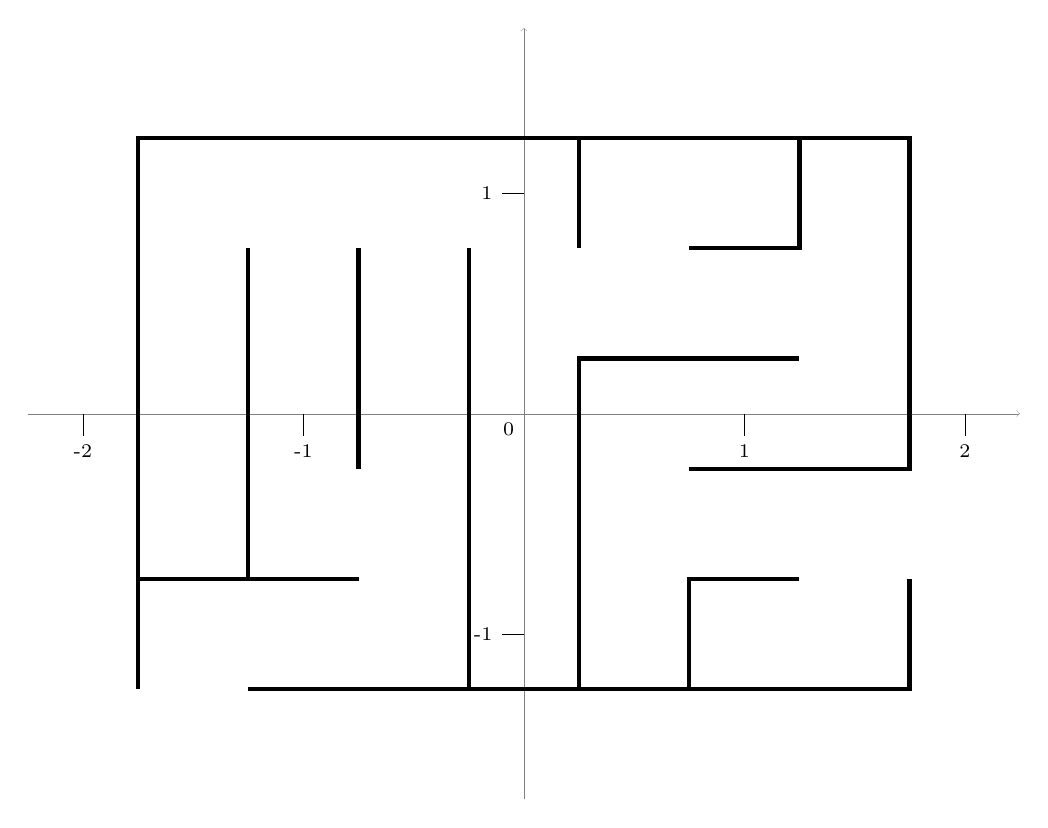
\begin{tikzpicture}[scale=2.8]
		\draw[gray,ultra thin,->] (-2.25,0) -- (2.25,0);
		\draw[gray,ultra thin,->] (0,-1.75) -- (0,1.75);
		\node[below left] at (0,0) {\scriptsize 0};

		\draw[very thin] (-2,0) -- ++(0,-0.1) node[below] {\scriptsize -2};
		\draw[very thin] (-1,0) -- ++(0,-0.1) node[below] {\scriptsize -1};
		\draw[very thin] (1,0) -- ++(0,-0.1) node[below] {\scriptsize 1};
		\draw[very thin] (2,0) -- ++(0,-0.1) node[below] {\scriptsize 2};

		\draw[very thin] (0,-1) -- ++(-0.1,0) node[left] {\scriptsize -1};
		\draw[very thin] (0,1) -- ++(-0.1,0) node[left] {\scriptsize 1};

		\draw[ultra thick] (-1.75,-1.25) -- ++(0,2.5) -- ++(3.5,0) -- ++(0,-1.5) -- ++(-1,0);
		\draw[ultra thick] (-1.25,-1.25) -- ++(3,0) -- ++(0,0.5);
		\draw[ultra thick] (-1.75,-0.75) -- ++(1,0);
		\draw[ultra thick] (-1.25,-0.75) -- ++(0,1.5);
		\draw[ultra thick] (-0.75,-0.25) -- ++(0,1);
		\draw[ultra thick] (-0.25,-1.25) -- ++(0,2);
		\draw[ultra thick] (0.25,-1.25) -- ++(0,1.5) -- ++(1,0);
		\draw[ultra thick] (0.75,-1.25) -- ++(0,0.5) -- ++(0.5,0);
		\draw[ultra thick] (0.25,1.25) -- ++(0,-0.5);
		\draw[ultra thick] (1.25,1.25) -- ++(0,-0.5) -- ++(-0.5,0);

		% \directlua{print_path(points)}
	\end{tikzpicture}
}

\newpage

\Paste{beta}

\end{document}